% TAAI 2026, international track. Springer LNCS, A4, 6--11 pages incl. references.
% Single-blind: author names and affiliations ARE shown.
%
% Build: pdflatex main; bibtex main; pdflatex main; pdflatex main
% Overleaf: choose the "Springer LNCS" template, then replace its main.tex with
% this file and upload the sec*.tex files and refs.bib alongside.

\documentclass[a4paper,runningheads]{llncs}

\usepackage[T1]{fontenc}
\usepackage{lmodern}
\usepackage{graphicx}
\usepackage{booktabs}
\usepackage{color}      % \UrlFont below needs \color; hyperref does not supply it
\usepackage{hyperref}
\hypersetup{hidelinks,
  pdftitle={Recoverable Error in Neural Climate Compression: A Rate-Matched Study of CRA5 over CONUS},
  pdfauthor={Tong-Jen Wang; Chieh-An Chou; Lu-Hung Chen}}
\usepackage{marvosym}   % \Letter, the envelope marking the corresponding author
\renewcommand\UrlFont{\color{blue}\rmfamily}

% The credits environment and its two names arrived in llncs 2023. Overleaf's
% template may predate that, and a missing \begin{credits} is a hard build error
% rather than a warning, so define them if absent.
\makeatletter
\@ifundefined{ackname}{\newcommand{\ackname}{Acknowledgments.}}{}
\@ifundefined{discintname}{\newcommand{\discintname}{Disclosure of Interests.}}{}
\@ifundefined{credits}{\newenvironment{credits}{\begingroup\small}{\endgroup}}{}
\makeatother

\begin{document}

\title{Recoverable Error in Neural Climate Compression:
       A Rate-Matched Study of CRA5 over CONUS}
\titlerunning{Recoverable Error in Neural Climate Compression}

% Single-blind track: names and affiliations are shown.
% Add verified ORCIDs only; placeholder identifiers should not appear in a
% submission. \authorrunning goes in the running head, so it stays short.
\author{Tong-Jen Wang \and
        Chieh-An Chou \and
        Lu-Hung Chen\textsuperscript{(\Letter)}}
\authorrunning{T.-J. Wang, C.-A. Chou, and L.-H. Chen}
\institute{National Chung Hsing University, Taichung, Taiwan\\
\email{g115018005@mail.nchu.edu.tw, st7110018036@gmail.com,\\
luhung@email.nchu.edu.tw}}

\maketitle

% LNCS asks for 150-250 words. Run wordcount.py after any edit to this block --
% it came in at 255 once and the limit is enforced by the template, not by taste.
\begin{abstract}
Learned atmospheric compressors are usually assessed by aggregate distortion,
which does not reveal how much residual error remains predictable from decoded
fields. We apply a fixed 1.65\,M-parameter U-Net to CRA5 reconstructions over
CONUS without adding per-frame bits. On the full 2018 test year, mean normalised
RMSE decreases by 25.8\% over 19 directly represented FourCastNet variables
(95\% temporal block-bootstrap interval [25.32, 26.18]\%). On the complete
2022 year outside CRA5's published training window, the same frozen checkpoint
and normalisation give a 26.4\% reduction [25.90, 26.93]\%, without fine-tuning.
Near-surface versus upper-air gains are 32.2\% versus 3.5\% in 2018 and 32.8\%
versus 3.6\% in 2022. A mean-rate-matched MPCA-only control has a smaller
near/upper gain ratio, while additional MPCA+PCA controls are explicitly
non-matched. A parameter-matched dilation ablation retains a roughly eightfold split
and concentrated gradient sensitivity. Using actual ERA5 orography and land--sea mask, western-land gains
rise from 18.1\% to 36.9\% across terrain-roughness endpoint deciles, although
residual error remains larger on rough ground. Earlier proxy-elevation controls
reduce an apparent 3.23-fold mountain error ratio to 1.14, showing substantial
spatial confounding. These results measure model-relative predictability;
terrain causality, corrector architecture effects, and broader distribution-shift
robustness remain open. Shared weights and inference add deployment costs.
\keywords{Scientific data compression \and Atmospheric reanalysis \and
Learned compression \and Decoder-side residual prediction \and ERA5}
\end{abstract}

\section{Introduction}
\label{sec:intro}

ERA5~\cite{hersbach2020} exceeds 400\,TB in float32, making storage and data
movement practical constraints. CRA5~\cite{han2024,cra5journal} uses a transformer
variational autoencoder to reduce this archive to about 0.85\,TB. Its published
evaluation describes reconstruction error by variable, pressure level, spatial
location, and spectrum. A separate question is how much error remains predictable
from the decoded fields themselves.

We attach a 1.65\,M-parameter U-Net to CRA5's decoded output.\footnote{Code and reproducibility: \url{https://github.com/tj567356/CRA5-Decoder-Correction}.}
On the 2018 CONUS test year, mean normalised RMSE (nRMSE) decreases by 25.8\% over the 19
FourCastNet variables directly represented by CRA5, without changing the
per-frame bitstream. Including derived total column water vapour gives 27.8\%.
We call this reduction \emph{model-recoverable error}: it depends on the chosen
network and training protocol and is not an information-theoretic bound.
On the complete 2022 year outside CRA5's published training window, the same
frozen corrector reduces direct-channel nRMSE by 26.4\% without fine-tuning.

The reduction is uneven: 32.2\% for near-surface fields versus 3.5\% aloft.
Their 9.1-fold ratio compares correction gains, not compression ratios. We apply
the same correction architecture, with separately fitted weights, to classical
transform codecs. A single-stage MPCA-only codec matched to CRA5's mean bits per
value gives a near/upper gain ratio of 1.7; three MPCA+PCA settings at higher
compression give 1.32--1.35. These controls help assess whether the asymmetry is
specific to the tested codec and corrector combination.

Terrain is a plausible contributor: small-scale topography may be difficult
to represent on a coarse latent grid, but error magnitude and correction gain
are different quantities. Using actual ERA5 orography and land--sea masks, we
find larger baseline errors and larger gains on rougher western land: $G$ rises
from 18.1\% to 36.9\% between roughness endpoint deciles. The association
persists within several elevation bands but does not isolate a terrain mechanism.
Our earlier proxy-elevation analysis remains a sensitivity check.

We contribute (i) a CRA5/MPCA comparison using measured bitstreams at
matched mean rate, distinguishing global and regional coding; (ii) vertical
recoverability with frozen 2022 testing and corrector controls; and (iii)
ERA5-orography roughness associations with elevation and geographic checks.
Checkpoints are selected on 2017 data; temporal block-bootstrap intervals
condition on each fitted model and test year.


\section{Related Work}
\label{sec:related}

CRA5~\cite{han2024,cra5journal} reports per-variable and per-level errors,
climatological bias maps, zonal spectra, and surface-station comparisons. Its
descriptor associates elevated error over mountain regions with topography.
Mirowski et al.~\cite{mirowski2024} provide elevation and a land--sea mask to a
reanalysis encoder. These results motivate terrain diagnostics, but spatial
association alone does not isolate terrain effects or decoder-side predictability.
Ding et al.~\cite{xu2025} evaluate CRA5 for vertically integrated tropospheric
delay, a different target from the horizontal residual structure studied here.

Decoder post-processing has precedent. Madireddy et al.~\cite{madireddy2021}
correct JPEG-compressed scientific simulation images with convolutional networks;
Jian et al.~\cite{jian2025} correct classical error-bounded compressors using a
3D CNN. Zhu et al.~\cite{zhu2026} correct frozen learned compressors by storing a
quantised residual, while NeurLZ~\cite{neurlz} also adds per-block information.
Our corrector stores no per-frame residual and has no pointwise error guarantee.

Alhumaidi et al.~\cite{alhumaidi2026} use CRA5, GraphCast, and Aurora as
predictors within an error-bounded pipeline sharing SZ3.1's backend. Their
residual maps and entropy analysis measure the cost of coding the remaining
error; our experiment measures how much a fixed model can predict from decoded
fields. These are complementary questions. Transform, quantisation, and entropy
coding are standard components of scientific codecs, including
TTHRESH~\cite{ballester2019}; the survey in~\cite{survey2025} provides broader
context. Our focus is the distribution of decoder-side correction gains, rather
than a general ranking of neural and classical compressors.

\section{Experimental Setup}
\label{sec:setup}

\subsection{Data and Metric}
ERA5~\cite{hersbach2020} is represented on a regular $0.25^\circ$
latitude--longitude grid and cropped to $25$--$49^\circ$N and
$130$--$70^\circ$W ($97\times241$ cells). We use the
20 FourCastNet variables~\cite{pathak2022}: five surface fields; winds and
geopotential at 1000/850\,hPa; temperature and relative humidity at 850\,hPa;
wind, geopotential, temperature, and relative humidity at 500\,hPa; geopotential
at 50\,hPa; and total column water vapour. Frames are six-hourly at 00/06/12/18
UTC. Training uses 2014--2016 (4{,}384 frames), validation 2017 (1{,}460), and
evaluation 2018 (1{,}460). Architecture and codec parameters are selected using
validation data; reported quantisation steps are fixed before 2018 evaluation.
The full-year 2022 test uses all 1{,}460 timestamps, January 1 at 00 UTC through
December 31 at 18 UTC. ERA5 truth combines 18 native
ARCO-ERA5 fields with native NCAR relative humidity at 500/850\,hPa; decoded
CRA5 and truth timestamps, coordinates, and channel order are checked exactly.
Source packing precision is cross-checked against 2018 samples. The original
checkpoint and 2014--2016 statistics are frozen; neither test year is used for
fine-tuning or selection.

We compute channel nRMSE as $\sqrt{\langle(x_j-\hat x_j)^2\rangle}/\sigma_j$.
The mean pools test times and cells; $\sigma_j$ is the training standard deviation. We
average these channel errors equally. Primary CRA5 means use 19 direct channels;
the full 20-channel mean is labelled separately. CRA5 does not store total column
water vapour (\texttt{tcwv}); we derive it by pressure integration of specific
humidity, truncated at the surface. Its $-0.63\,\mathrm{kg\,m^{-2}}$ bias can
be learned by the corrector, so its gains partly repair this derivation.

For channel errors $b_j$ before and $a_j$ after correction, the headline reduction
is $G=1-\sum_j a_j/\sum_j b_j$. Equal-weight fractional gain is
$\bar G=p^{-1}\sum_j(1-a_j/b_j)$. The former weights fractional gains by baseline
error; the latter treats channels equally. Terrain roughness uses $G$; the legacy proxy-elevation control instead uses
$G_{\mathrm{pool}}$ (Section~\ref{sec:terrain}).

\subsection{Correction Network}
\label{sec:cnn}
All correctors train with 20 input/output channels; direct19 is only an evaluation
subset. U-Net depth is 2, base/bottleneck widths 64/128, with $3\times3$
convolutions and 1{,}646{,}548 parameters. Input is $(\hat x-\mu)/\sigma$,
target $(x-\hat x)/\sigma$, and corrected field $\hat x+\sigma f(\cdot)$;
$\mu,\sigma$ are fixed training statistics. CRA5 correction minimises normalised
residual MSE using AdamW: learning rate $3\times10^{-4}$, weight decay $10^{-4}$,
gradient clipping 1.0, batch 8, mixed precision, seed 0, maximum 200 epochs,
and early-stopping patience 12. The architecture comes from a 33-configuration
MPCA sweep ranked on 2017, not a CRA5 architecture search. Classical checkpoints
share the architecture/objective but not identical budgets: inspected MPCA-only
and e995 logs allow 200 and 100 epochs. Each is reused without retraining here.

We decode the released CRA5 streams for 2014--2018 and extract CONUS.
Baseline 20-channel nRMSE ranges from 0.08523 to 0.08752 across these years;
they overlap CRA5 training (Section~\ref{sec:limitations}). New 2018 diagnostics
replay the original checkpoint with float32 inference on the existing float16
normalised cache and float64 aggregation, reproducing original rounded results.

\subsubsection{Temporal uncertainty.}
Squared-error sums and counts for each frame and channel support a paired circular
moving-block bootstrap: 28-frame (seven-day) blocks wrap at the year boundary,
with each draw truncated to 1{,}460 frames. In 1{,}000 draws (seed 20261026),
before/after errors share sampled timestamps; channel RMSEs and $G$ are recomputed.
Percentile 95\% intervals condition on checkpoint, year, and grid, excluding
training-seed and spatial uncertainty. The same protocol is applied to 2022.

\section{A Rate-Matched Classical Encoder}
\label{sec:encoder}

The classical control uses multilinear PCA independently for each channel. Separate
latitude and longitude bases retain 99\% energy per axis; a core $C$ reconstructs
as $LCR^{\!\top}$. The twenty channels together retain 10{,}193 coefficients per
frame. MPCA-only quantises these directly. MPCA+PCA adds a global PCA: e995, e99,
and e97 retain 99.5\%, 99\%, and 97\% energy, yielding 2{,}011, 1{,}449, and
636 components, respectively.

A uniform step $\Delta$ quantises the coefficients; a range coder uses a
zero-mean Gaussian model with training-estimated scale for each coefficient.
Every configuration is checked by an exact integer round-trip. All compression
ratios (CRs) use measured coded bytes, not coefficient counts. For example,
2{,}011 float32 coefficients imply $232\times$, whereas the measured e995 stream
achieves $1333\times$. Larger CR means lower bits per source value,
$R=32/\mathrm{CR}$.

The reported MPCA rate includes the scale table amortised over 7{,}304 frames
(5.58 bytes per frame for MPCA-only). Transform bases are fixed codec parameters,
as CRA5 weights are, and excluded from the per-frame payload. MPCA-only's bases
contain 153{,}682 floats; including their amortised 84 bytes per frame would
change its CR to approximately $463\times$. MPCA+PCA additionally requires a
fixed global basis. These shared costs matter for short archives.

CRA5's 2018 streams average 2{,}360{,}056 bytes for
$721\times1440\times268$ float32 values: $471.60\times$, or 0.0679 bits per value.
Matching this rate for our $20\times97\times241$ fields gives 3{,}965.6 bytes per
frame. Bisection on 2017 coded sizes fixes $\Delta=0.7659$; the frozen step yields
3{,}952.9 bytes and $473.12\times$ on 2018, a 0.3\% rate mismatch.

Figure~\ref{fig:main}'s matched MPCA+PCA retains 4{,}384 components, distinct
from e995/e99/e97. Matching concerns \emph{mean bits per source value}. CRA5 jointly codes 268 global
channels; MPCA is fitted to 20 regional channels. Their domains and coding tasks
are different, and the global bitstream cannot identify CRA5's exact cost for
this regional subset. The comparison is an operating-point control, not an
equivalent-domain benchmark. MPCA-only is the main matched-rate classical control.

\section{Results at Matched Rate}
\label{sec:results}

Figure~\ref{fig:main} uses validation-selected quantisation; the 0.3\% rate
mismatch slightly favours CRA5. Correctors share an architecture/objective,
with compressor-specific weights. Classical correctors train before quantisation
and evaluate after it; CRA5 uses decoded streams throughout. Quantisation changes
classical corrected nRMSE by 0.07--0.44\%, but the mismatch remains a limitation.

\begin{figure}[t]
\centering
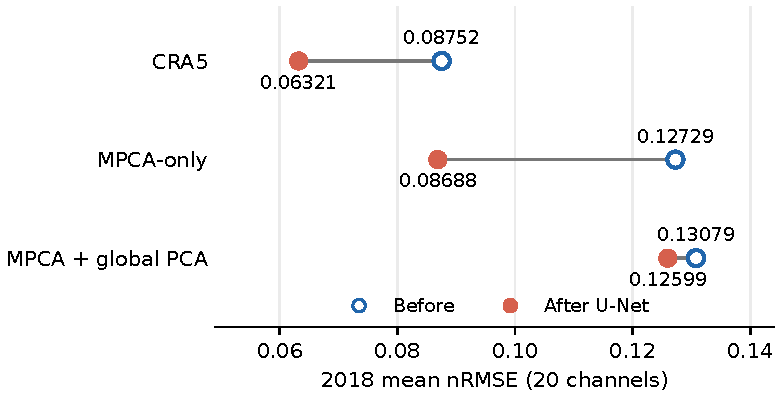
\includegraphics[width=0.90\textwidth]{figs/main_result}
\caption{Matched mean 2018 rates: CRA5 $471.6\times$, MPCA-only $473.1\times$,
and MPCA+global-PCA $472.9\times$. Hollow markers denote baseline and filled
markers add correction without per-frame bits. Values average all 20 channels,
including derived \texttt{tcwv}, matching the 20-channel columns in
Table~\ref{tab:outtime}.}
\label{fig:main}
\end{figure}

CRA5 has lower error before and after correction (Fig.~\ref{fig:main}).
Corrected MPCA-only (0.08688) is only 0.73\% below uncorrected CRA5 (0.08752);
different post-processing prevents a decisive compressor ranking.
At matched rate, global PCA raises corrected error by 45\% versus MPCA-only.

\subsubsection{Decoder-side repair.}
\label{sec:zerobit}
CRA5 direct19 nRMSE falls from 0.08661 to 0.06431
($G=25.8\%$, $\bar G=19.3\%$). With derived \texttt{tcwv}, $G=27.8\%$.

The unchanged bitstream requires no residual side information;
shared correction weights cost about 6.6\,MB in float32 plus inference computation.
This is model-relative predictability, not an information-theoretic bound.
Profiling counts 19.86\,G FLOPs per frame. On an RTX 3080,
float32 GPU-resident inference at batch 8 averages 1.32\,ms per frame with TF32
allowed; this excludes decoder, I/O, and transfer costs.

The 95\% bootstrap intervals for direct19, near and upper $G$ are
[25.32, 26.18]\%, [31.73, 32.62]\% and [3.38, 3.68]\%, respectively. The near-minus-upper difference
is 28.66 percentage points [28.31, 29.01]. Table~\ref{tab:asymmetry} gives group
errors; intervals condition on checkpoint, year and grid.

\subsubsection{Full-year out-of-time evaluation.}
Unlike 2018, the complete 2022 test year is outside CRA5's published training
window. Table~\ref{tab:outtime} shows that the frozen corrector retains its
aggregate improvement: direct-channel $G=26.40\%$ with a 95\% block-bootstrap
interval of [25.90, 26.93]\%. Near-surface gain is 32.79\% [32.28, 33.31]\%
versus 3.60\% [3.46, 3.76]\% aloft, a 9.10-fold ratio.

\begin{table}[t]
\centering
\caption{Full-year CRA5 correction, 1{,}460 frames/year. After$_{20}$ and $G_{20}$
include derived \texttt{tcwv}, matching Fig.~\ref{fig:main}; baseline nRMSE is
0.08752/0.08700 in 2018/2022. All $G$ columns are percentage reductions:
$G_{19}$ excludes \texttt{tcwv}; $G_N,G_U$ use near13/upper6. All checkpoints
are 2017-selected and frozen. Dilated is parameter-matched; Affine is not.}
\label{tab:outtime}
\begin{tabular}{llr@{\hspace{1.5em}}rrrr}
\toprule
Corrector & Year & After$_{20}$ & $G_{20}$ & $G_{19}$ & $G_N$ & $G_U$ \\
\midrule
U-Net & 2018 & 0.06321 & 27.78 & 25.75 & 32.18 & 3.52 \\
 & 2022 & 0.06236 & 28.32 & 26.40 & 32.79 & 3.60 \\
Dilated & 2018 & 0.06354 & 27.40 & 25.38 & 31.61 & 3.82 \\
 & 2022 & 0.06270 & 27.93 & 26.01 & 32.21 & 3.91 \\
Affine & 2018 & 0.08471 & 3.20 & 1.29 & 1.43 & 0.82 \\
 & 2022 & 0.08425 & 3.16 & 1.31 & 1.45 & 0.85 \\
\bottomrule
\end{tabular}
\end{table}

Including derived \texttt{tcwv}, 2022 nRMSE is 0.08700 before and 0.06236 after
correction ($G=28.32\%$); \texttt{tcwv} alone gains 59.43\%. Aggregate gains
do not imply uniform improvement: $v500$ worsens slightly (gain $-0.0082\%$).

\section{Where the Error Lives}
\label{sec:where}

\subsubsection{Field altitude and variable identity.}
Near-surface means surface fields plus 1000/850\,hPa (13 channels); upper-air
means 500/50\,hPa (6). These refer to field altitude, not ground elevation;
\texttt{tcwv} spans the atmospheric column and belongs to neither group.
The reductions are $G=32.2\%$ versus $3.5\%$ and $\bar G=27.5\%$ versus
$1.5\%$. Their ratios, 9.1 and 18.6, compare gains rather than compression.
Surface-pressure nRMSE falls from 0.0990 to 0.0249; the 500\,hPa wind errors
are unchanged to four decimals. The largest upper-air gain is 7.4\% for relative
humidity at 500\,hPa.

Across 1000, 850 and 500\,hPa, $u$ gains are 40.5\%, 20.1\% and approximately
zero; $v$ gives 40.7\%, 19.6\% and approximately zero. From 850 to 500\,hPa,
$t$ falls from 12.3\% to 0.1\%, $r$ from 15.1\% to 7.4\%: variable identity alone
does not explain the split.
\begin{table}[t]
\centering
\caption{Full-2018 frozen-checkpoint evaluation (1{,}460 frames). Before/after
nRMSE averages 13 near-surface or 6 upper-air direct channels; both exclude
column-integrated \texttt{tcwv}. $G$ is their relative reduction. CR uses measured entropy-coded bytes: R is CRA5 reference,
M is matched mean rate, and N is non-matched. e995/e99/e97 denote MPCA+PCA.
Each system reuses its own previously trained weights; MPCA-only was trained on
stage-1-only reconstruction and is not retrained for this table. Classical rows
use actual quantised reconstruction at the original fixed steps.}
\label{tab:asymmetry}
\begin{tabular}{lllrr@{\hspace{2em}}r}
\toprule
System & CR/status & Group & Before & After & $G$ (\%) \\
\midrule
CRA5 & 471.6 R & Near & 0.09820 & 0.06660 & 32.18 \\
 & & Upper & 0.06151 & 0.05934 & 3.52 \\
MPCA-only & 473.1 M & Near & 0.12913 & 0.08207 & 36.44 \\
 & & Upper & 0.12289 & 0.09690 & 21.14 \\
e995 & 1333 N & Near & 0.17983 & 0.14221 & 20.92 \\
 & & Upper & 0.15849 & 0.13392 & 15.50 \\
e99 & 2000 N & Near & 0.19156 & 0.15536 & 18.89 \\
 & & Upper & 0.17149 & 0.14686 & 14.36 \\
e97 & 5093 N & Near & 0.22290 & 0.19081 & 14.39 \\
 & & Upper & 0.20767 & 0.18505 & 10.89 \\
\bottomrule
\end{tabular}
\end{table}

\subsubsection{Classical controls and architecture.}
Near/upper $G$ ratios are 9.14 for CRA5, 1.72 for matched MPCA-only, and
1.32--1.35 for non-matched MPCA+PCA (Table~\ref{tab:asymmetry}). Distinct
checkpoint weights share an architecture and residual objective. This supports
a compressor-dependent pattern for this corrector, but its local receptive field
may preferentially repair surface structure while missing broader upper-air
errors. The MPCA architecture sweep does not isolate CRA5 receptive-field effects;
we therefore test a fixed parameter-matched intervention below.

\subsubsection{Parameter-matched receptive-field ablation.}
DilatedUNet2 changes only the two bottleneck convolutions to dilation/padding
2 and 3, preserving all other operations, shapes and 1{,}646{,}548 parameters.
The same CRA5 residuals and training recipe select epoch 125 on 2017, stopping
at 137 before testing. This fixed ablation is not architecture search.
Training/validation takes 2{,}278\,s. Both models use 19.86\,G counted
FLOPs/frame; same-run batch-8 inference averages 1.316/1.315\,ms/frame.

Including pooling, bilinear resizing and skips, central theoretical support
grows $72\times72\to96\times96$ cells (unclipped maximum spans 76\,$\to$\,100
per axis). Gradient diagnostics of $f(x)$ use eight fixed 2017 inputs, all 20
outputs and three positions: 480 probes/model. Squared gradients are summed
over input channels and each probe normalised. Central mean 90\%-energy Chebyshev radius decreases
3.41\,$\to$\,2.78 cells. Across all probes, mean Dilated energy outside the
original support is only 0.0033\%. Expanded theoretical support does not imply broad effective use.

Overall correction is slightly worse (Table~\ref{tab:outtime}). In 2018/2022,
upper $G$ rises 0.30/0.31 percentage points (paired 95\% intervals [0.27,0.33]/[0.28,0.34]),
while near $G$ falls 0.57/0.58 points. Near/upper ratios remain 8.28/8.24;
differences are 27.79/28.30 points. $z500$ worsens ($G=-4.46\%/-5.12\%$),
and upper $\bar G$ falls to 0.94\%/1.01\%. This ablation retains the split,
but concentrated gradients and one seed leave broader architecture effects open.

\subsubsection{Low-capacity affine control.}
One $3\times3$ convolution (20\,$\to$\,20, bias, no activation) has 3{,}620
parameters: \emph{not parameter-matched}. The same recipe selects epoch 125 on
2017, stopping at 137; frozen direct19 gains are only 1.29\%/1.31\% in
2018/2022. Its 2018 upper $\bar G=-0.91\%$. Different capacity and context
prevent attributing the U-Net gap solely to nonlinearity.

\subsubsection{Spatial diagnostic.}
For a $5\times5$ box smoother $S_5$, fine-scale error fraction
$\mathrm{Var}(e-S_5(e))/\mathrm{Var}(e)$ is 57.6\%/27.6\% near/upper for CRA5,
versus 22.2\%/5.5\% for unquantised e995. This diagnostic does not establish a mechanism.

\section{Testing the Terrain Hypothesis}
\label{sec:terrain}

Larger reconstruction error need not imply a larger correctable fraction. We
compare both against actual-orography roughness and retain the original
proxy-elevation comparison as a sensitivity check.

\subsubsection{Actual orography and roughness.}
ERA5 surface geopotential and land--sea mask are extracted from ARCO-ERA5 at
2018-01-01 00 UTC, with coordinates checked against the original $97\times241$
grid. Elevation is geopotential divided by $9.80665\,\mathrm{m\,s^{-2}}$; land
is $\mathrm{lsm}>0.5$. Roughness is population elevation standard deviation in a
$5\times5$ land-only neighbourhood with at least 13 valid neighbours. Ocean and
out-of-domain cells are excluded without padding. Excluding 102 land cells leaves
15{,}343 cells overall and 7{,}573 west of $100^\circ$W.

Ten terrain-only quantile bins per region fix identical cells before and after
correction. Per-channel normalised squared error is pooled over bin cells and
all 1{,}460 test frames, square-rooted, then averaged over the 19 direct channels.
The frozen checkpoint and 2014--2016 normalisation are unchanged.

\begin{figure}[t]
\centering
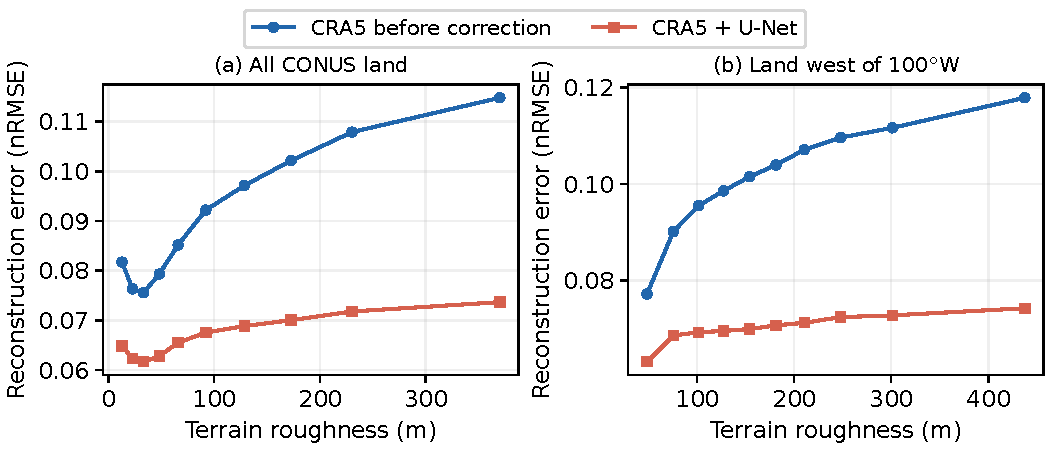
\includegraphics[width=\textwidth]{figs/terrain_roughness_main_curve}
\caption{2018 frozen U-Net errors: 19 direct channels, 2014--2016 normalisation.
Roughness is $5\times5$ land-only elevation SD with at least 13 valid neighbours.
Points are ten region-specific quantile bins at mean roughness; lines connect
measurements. Both curves use identical cells/timestamps within each panel.
Western land controls east--west composition; association does not imply causality.}
\label{fig:roughness}
\end{figure}

Figure~\ref{fig:roughness} shows larger baseline errors on rougher ground,
except for a non-monotone low-roughness segment on all land. Between endpoint
all-land deciles, baseline nRMSE rises from 0.08170 to 0.11482 and corrected
nRMSE from 0.06479 to 0.07364; $G$ rises from 20.7\% to 35.9\%. On western
land, baseline nRMSE rises from 0.07724 to 0.11783. Corrected error rises from
0.06323 to 0.07430; $G$ increases from 18.1\% to 36.9\%. Correction narrows but
does not remove the error gradient. All-land near-surface gain rises from 26.1\%
to 43.6\%; upper-air gains remain 3.1--3.7\% across deciles.

\subsubsection{Elevation controls.}
Roughness/elevation Spearman correlation is 0.694 overall and 0.265 on western
land. Western comparisons within fixed elevation bands (0--200, 200--600,
600--1200, 1200--2000, and above 2000\,m) retain the broad association in several
bands. For example, $G$ rises from 14.3\% to 36.8\% across endpoint deciles
at 600--1200\,m. The pattern is not uniform: 0--200\,m gains fluctuate around
30--35\%, with only 29--31 cells per bin. These are descriptive controls, not
independent spatial replications.

\subsubsection{Original proxy-elevation sensitivity.}
Table~\ref{tab:twoheights} retains the original comparison at fixed western
proxy-land positions.

\begin{table}[!htb]
\centering
\caption{Original elevation control, western proxy-land, 2018: identical ground
grid columns for near13/upper6, excluding \texttt{tcwv}. Gains are
$1-\sqrt{\langle a^2\rangle/\langle b^2\rangle}$, where $a,b$ are per-cell
normalised RMSE after/before correction; averaging pools channels and cells.
This differs from $G,\bar G$; ratios use unrounded gains.}
\label{tab:twoheights}
\begin{tabular}{lrrrr}
\toprule
Elevation band & Cells & Near & Upper & Ratio \\
\midrule
0--200\,m & 415 & 39.9\% & 5.0\% & 7.9$\times$ \\
200--600\,m & 850 & 39.2\% & 5.2\% & 7.6$\times$ \\
600--1200\,m & 2{,}311 & 33.5\% & 4.7\% & 7.1$\times$ \\
1200--2000\,m & 3{,}113 & 40.1\% & 4.7\% & 8.6$\times$ \\
above 2000\,m & 984 & \textbf{41.9\%} & \textbf{4.3\%} & \textbf{9.7$\times$} \\
\bottomrule
\end{tabular}
\end{table}

The pressure-derived standard-atmosphere elevation and 1.0\,K diurnal
2\,m-temperature land threshold differ from the actual static fields above.
The baseline surface-pressure high/low-elevation error ratio is $3.23\times$
over CONUS, $2.28\times$ on proxy-land, and $1.14\times$ on western proxy-land;
MPCA+PCA e995 gives 2.09, 1.70, and 0.95. This negative result is retained:
mean elevation differs from roughness, and the original gradient is strongly
confounded by land/sea and longitude.

Above 2000\,m, eight low-level channels may include below-ground ERA5
extrapolation, potentially easing prediction. Proxy-sea gains also differ,
23.9\% versus 5.5\%: ground location alone does not explain the split.

\section{Limitations}
\label{sec:limitations}

CRA5 reportedly trained on 1979--2021 and tested on 2022--2023~\cite{han2024};
we did not audit its checkpoint log. Our 2018 test overlaps CRA5 training,
while one frozen 2022 test, one CONUS region, one neural codec and few
correctors do not establish broad generalisation.

Matched mean rates compare different global/regional coding tasks. Frame-rate
coefficients of variation are 0.95\% for CRA5 and 3.70\% for MPCA-only.
Payloads exclude shared bases and correction weights; inference adds cost.
Derived \texttt{tcwv} includes derivation error. No pointwise or per-block
improvement is guaranteed.

Seven-day bootstrap intervals condition on checkpoint, year and grid; they do
not remove all temporal or spatial dependence. Roughness covaries with elevation
and geography; western lowland bins have only 29--31 cells, while mountain
pressure levels may be below ground. Terrain associations are not causal.
One dilation pattern/seed cannot exclude broader context or optimisation effects;
unequal group sizes and error magnitudes affect the shared residual-MSE loss.

\section{Conclusion}
\label{sec:conclusion}

A frozen U-Net lowers CRA5 direct19 nRMSE by 25.8\% (2018) and 26.4\%
(unseen 2022) without extra frame bits. Near/upper gains are 32--33\% versus
3.5--3.6\%, a split retained by parameter-matched dilation with slightly
worse overall error. On western land, terrain roughness correlates with
higher baseline errors and correction gains; corrected errors remain higher
and elevation controls do not establish causality. Model-relative recovery
persists in one unseen year; broader robustness, architecture effects and
inference costs remain limitations.


% LNCS 2023 onward requires both of the following, in this order, as bold run-in
% headings in small font. The disclosure is mandatory even when there is nothing
% to disclose.
\begin{credits}
\subsubsection{\discintname}
The authors have no competing interests.
\end{credits}

\bibliographystyle{splncs04}
\bibliography{refs}

\end{document}




